\chapter{Natural Language Processing}
\thispagestyle{fancy}
\label{chap:Natural Language Processing}

\noindent
Natürliche Sprache wird auch als menschliche Sprache bezeichnet und ist historisch gewachsen. Sie verfolgt orthographische und grammatikalische Regeln auf Grundlage eines sprachabhängigen Wortschatzes. Die Sprachwissenschaft, auch Linguistik genannt, untersucht natürliche Sprache mithilfe verschiedener Methoden. \ac{NLP} meint die maschinelle Verarbeitung natürlicher Sprache. Dabei werden Methoden der Linguistik unter anderem mit Methoden des Deep Learning verknüpft \cite[S.~1]{BIR09}. Nicht selten ist eine Spracherkennung vorgeschaltet. \ac{NLP} ist weiterhin in \ac{NLU} und \ac{NLG} zu untergliedern \cite[S.~27-28]{BIR09}. Diese Teilgebiete sind zugleich wesentliche Herausforderungen der \ac{ATS}.\\

\noindent
\ac{NLP}-Aufgaben sind oftmals als Optimierungsprobleme zu verstehen. Lösungen sind demnach nicht eindeutig, also im mathematischen Sinne analytisch nicht lösbar. Dies wird in Hinblick auf die \ac{ATS} deutlich, wenn man verschiedene Personen den gleichen Text zusammenfassen lässt. Zwar gleichen sich die als relevant identifizierten Informationen größtenteils, doch die Formulierungen sind mitunter sehr unterschiedlich. Folglich können auch mehrere Versionen korrekt sein.\\

\noindent
Natürliche Sprache bedarf hinsichtlich maschineller Verarbeitung einer geeigneten mathematischen Form. Hierfür werden nachfolgend verschiedene Vorverarbeitungsschritte sowie Word Embeddings und Deep Language Representations vorgestellt. Der Anspruch auf Vollständigkeit entfällt aufgrund der Mächtigkeit des \ac{NLP}, obgleich anknüpfende Inhalte bei Bedarf an den entsprechenden Stellen erläutert werden.
\newpage


\section{Vorverarbeitung}
\noindent
In nahezu allen Teilbereichen der Data Science stehen gewöhnlicherweise etliche Vorverarbeitungsschritte an, um die zu analysierenden Daten zu bereinigen, zu normalisieren und insgesamt in eine konsistente sowie geeignete Form zu bringen. Im \ac{NLP}-Kontext sind indes komplexere Vorverarbeitungsschritte erforderlich, um die Daten für die eingeforderte mathematische Form zu präparieren \cite[S.~86]{BIR09}. Eine Auswahl der in dieser Arbeit relevanten Schritte wird nachfolgend vorgestellt. In der Implementierung dieser chronologisch aufeinander folgenden Schritte spricht man auch von der \ac{NLP}-Pipeline.


\subsection{Textbereinigung}
\noindent
An erster Stelle der \ac{NLP}-Pipeline steht die Textbereinigung, welche sich bezüglich eingehender Sequenzen insbesondere auf Sonderzeichen, Interpunktion sowie Klein- und Großschreibung konzentriert. Dabei ist es mitunter bereits herausfordernd, entsprechende Textstellen als solche zu identifizieren. Anschließend sind oftmals normalisierende Maßnahmen anzuwenden. Üblich ist beispielsweise das Entfernen von Sonderzeichen oder auch das Erzwingen von Kleinschreibung in allen eingehenden Texten \cite[S.~107]{BIR09}. Weit verbreitet ist auch das Entfernen von Stoppwörtern. Dies sind Wörter, welche mutmaßlich der Allgemeinsprache zugehören, weshalb angenommen wird, dass sie keine entscheidende inhaltliche Bedeutung besitzen \cite[S.~5]{GAM16}. Hier lässt sich jedoch keine allgemeingültige Aussage treffen, da die tatsächlich erforderlichen Maßnahmen sowohl von den Eigenschaften der Eingangsdaten als auch von den Besonderheiten der verwendeten Modelle und den verfolgten Zielen abhängen. Dabei ist die Datenexploration wiederkehrend und alternierend mit der Anpassung der Vorverarbeitung auszuführen. Der Anwender sollte hierbei ein Gefühl für die Daten und deren Besonderheiten entwickeln. Zudem bedarf es einem tiefgründigen Verständnis der geplanten Aufgaben, um beurteilen zu können, welche Vorverarbeitungsschritte tatsächlich relevant sind.


\subsection{Textnormalisierung}
\noindent
In der weitergehenden Textnormalisierung wird sich vorrangig auf das Stemming und die Lemmatisierung konzentriert. Das Stemming führt eingehende Wörter auf ihre Grundformen zurück, indem bekannte Präfixe, Infixe und Suffixe eliminiert werden. Diese Grundformen sind nicht zwingend valide Wörter. Die Lemmatisierung hingegen berücksichtigt die wortspezifischen Bedeutungen, um etwaige Flexionen in Deckung zu bringen und somit die linguistisch korrekten Grundformen zu bilden. Flexionen sind durch Konjugationen, Deklinationen oder auch Komparationen entstanden und natürlicher Bestandteil einer Sprache. Hierfür sind Wortbildungsregeln und ein Wortschatz erforderlich. Letzterer indiziert die eingehenden Wörter anhand ihrer Lemmata und ordnet sie entsprechend zu \cite[S.~107-108]{BIR09}. Zwar ist die Lemmatisierung aufgrund des erforderlichen Kontextwissens durchaus komplexer als das Stemming, dafür sind ihre Ergebnisse erwartungsgemäß gehaltvoller. Ob und welche Methode zur Textnormalisierung herangezogen wird, hängt erneut von der anvisierten Aufgabe ab. Seien nun beispielhaft die Wörter \{\textit{spielen, spielst, spielte, gespielt}\} gegeben, dann reduziert der Stemmer diese Wörter auf die Grundform \textit{spiel}. Der Lemmatizer identifiziert hingegen die linguistisch korrekte Grundform \textit{spielen}.\\

\noindent
\ac{NLTK} ist eine forschungsorientierte Python-Bibliothek, die etliche \ac{NLP}-Module zur Verfügung stellt, darunter unter anderem verschiedenartige Stemmer \cite[S.~13-14]{BIR09}. Stemmer, welche die englische Sprache unterstützen, scheinen bereits sehr ausgereift zu sein. Stemmer, welche die deutsche Sprache unterstützen, sind nicht nur knapp, sondern bedürfen zudem weitergehenden Testschritten, um deren tatsächliche Eignung zu prüfen. Die Stemmer nltk.stem.cistem und nltk.stem.snowball eignen sich potenziell für einen Einsatz mit deutscher Sprache \cite{NLT20}.\\

\noindent
SpaCy ist eine eher praktisch orientierte Python-Bibliothek für verschiedenste \ac{NLP}-Aufgaben. Hinsichtlich der deutschen Sprache eignen sich hier insbesondere die verfügbaren Lemmatizer. Dabei kann der Anwender zwischen verschiedenen vortrainierten Modellen wählen. Eigenschaften wie Sprache, Größe und zugrundeliegende Trainingsdaten sind transparent dokumentiert \cite{SPA21}.\\

\noindent
Die Wahl geeigneter Stemmer und Lemmatizer obliegt dennoch den subjektiven Präferenzen des jeweiligen Entwicklers. In jedem Fall sind hinreichende Tests durchzuführen, um die einzelnen Module zu erproben sowie individuelle Vor- und Nachteile zu identifizieren. Mit fortschreitender Entwicklung beweisen sich möglicherweise auch andere aufstrebende Bibliotheken \cite[S.~108]{BIR09}.
\newpage


\subsection{Tokenisierung}
\noindent
In der Tokenisierung werden Texte in logisch zusammengehörige Token zerlegt. Texte bestehen aus Sequenzen, welche wiederum aus Symbolen, also etwa Zeichen, Zeichenketten oder auch Ziffern bestehen. Token sind indes als Einheiten der Wort- oder Satzebene zu verstehen \cite[S.~22-24]{MAN08}.\\

\noindent
Der einfachste Ansatz einer wortbasierten Tokenisierung besteht darin, den Text anhand von Leerzeichen und nicht-alphanumerischer Zeichen zu segmentieren. Dies ist jedoch nicht völlig obligatorisch und führt meist nicht zu einer verarbeitbaren Lösung, weshalb sprachabhängige Eigenarten berücksichtigt werden müssen. Typisch ist beispielsweise die Weiterbehandlung von vor- oder nachstehenden Klammern an den Token \cite[S.~109-111]{BIR09}.\\

\noindent
Ob weiterhin auch Interpunktion berücksichtigt oder verworfen werden soll, ist hinsichtlich der anvisierten \ac{NLP}-Aufgabe individuell zu entscheiden und zu erproben. Gleiches gilt für die Entscheidung, ob eingehende Texte roh oder vorverarbeitet hineingegeben werden.\\

\noindent
Sei nun ein Satz gegeben, welcher keiner Textbereinigung und keiner Textnormalisierung unterzogen wird. Eine Tokenisierung, welche die Eigenschaften der deutschen Sprache sowie Interpunktion hinreichend berücksichtigt, würde die in \autoref{pic:Tokenization} visualisierte Menge von Token generieren.

\begin{figure}[h!]
  \centering
  \fbox{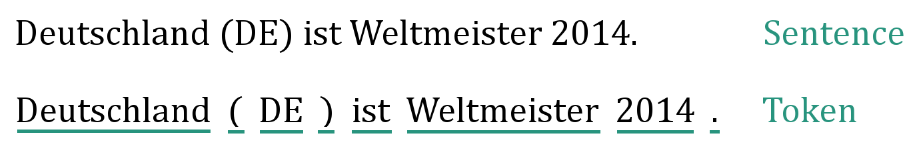
\includegraphics[width=0.6\linewidth]{./source/images/tokenization.png}}
  \caption{Tokenisierung eines beispielhaften Satzes.}
  \label{pic:Tokenization}
\end{figure}

\noindent
Die Arbeit mit Texten erfordert bekanntermaßen eine geeignete mathematische Form. Die zeichenbasierten Token der Texte werden daher in einem Wortschatz (engl. Vocabulary) mithilfe numerischer Indizes kodiert. Hier ist es möglich, die Anzahl eindeutiger Token zu identifizieren oder gar seltene Token aus praktischen Gründen zu entfernen \cite[S.~311-312]{ZHA20}.
\newpage

\noindent
Die Python-Bibliotheken \ac{NLTK} und SpaCy stellen entsprechende Tokenizer für eine möglichst schnelle Implementierung bereit. Beide sind überdies in einer für die deutsche Sprache ausgereiften Version verfügbar. Oftmals werden hierbei weitere Funktionalitäten mitgeliefert, darunter meist das Entfernen sprachbezogener Stoppwörter, die Lemmatisierung oder auch das Part-of-Speech-Tagging \cite[S.~111]{BIR09}.


\section{Word Embeddings}
\noindent
Algorithmen können Texte bekanntermaßen nicht in ihrer Rohform verarbeiten. Texte bedürfen einer geeigneten mathematischen Form. Word Embeddings überführen Texte oder ganze Korpora hierfür in einen Vektorraum (engl. Vector Space), um Wörter syntaktisch, semantisch und insbesondere untereinander in Kontext zu bringen. Dabei wird ein Wortschatz benutzt, welcher die entsprechenden Vektoren, bestehend aus eindeutig kodierbaren ganzzahligen Werten, aufbaut \cite{KAR18}. Die Ableitung der Vektoren aus den Textdaten wird auch als Feature Extraction oder Feature Encoding bezeichnet. Insgesamt befindet man sich hier im Bereich des Language Modeling \cite{BRO19}.\\

\noindent
Word Embeddings werden üblicherweise noch vor der Entwicklung der ursprünglich anvisierten \ac{NLP}-Aufgabe trainiert, weshalb ihnen ein unmittelbarer qualitativer Einfluss zugesprochen wird. Die entstehenden Modelle sind in der Folge schnell implementierbar. Weiterhin haben sie hiermit einen hohen skalierenden Effekt, da sie als Grundlage verschiedenster nachgelagerter \ac{NLP}-Aufgaben eingesetzt werden können \cite{NIT19}. Word Embeddings können durch verschiedene mehr oder minder komplexe Ansätze realisiert werden. Diese werden nachfolgend vorgestellt, wobei stets verdeutlicht wird, wie der entsprechende Vektorraum aufgebaut und in Kontext gebracht wird. Dabei wird außerdem deutlich, dass sich die verschiedenen Ansätze nicht für jede \ac{NLP}-Aufgabe eignen, sondern sie vielmehr einschränken. Obgleich nicht alle Ansätze für die \ac{ATS} relevant sein werden, sind sie als Grundlage zu verstehen.
\newpage


\subsection{One-Hot-Encoding}
\noindent
\ac{OHE} ist einer der einfachsten Ansätze, um Texte in einen Vektorraum einzubetten. Dabei werden allgemein kategorische Variablen in ein numerisches und somit mathematisch verarbeitbares Format gebracht \cite{KAR18}. Seien nun zwei gleichbedeutende Sätze gegeben. Eben jene Sätze sowie der entsprechende Wortschatz und die binär kodierten Vektoren sind in \autoref{pic:OneHotEncoding} ersichtlich. Die Vektoren sind hierbei als Matrix zusammengefasst, wobei die Zeilen und Spalten anhand der Anfangsbuchstaben der Wörter kenntlich gemacht sind.\\

\noindent
Versucht man nun, diese Vektoren in einem Vektorraum zu visualisieren, dann entspricht jeder Vektor einer eigenen Dimension. Dabei wird allerdings klar, dass keine dimensionsübergreifenden Projektionen existieren \cite{KAR18}. Dies bedeutet, dass die Wörter \textit{gutes} und \textit{schönes} genauso verschieden sind, wie die Wörter \textit{heute} und \textit{ist}. Dies ist offensichtlich falsch. \ac{OHE} ist dennoch als Grundlage zu verstehen, wobei etwaige Probleme innerhalb der nachfolgenden Ansätze weiterbehandelt werden.\\

\begin{figure}[h!]
  \centering
  \fbox{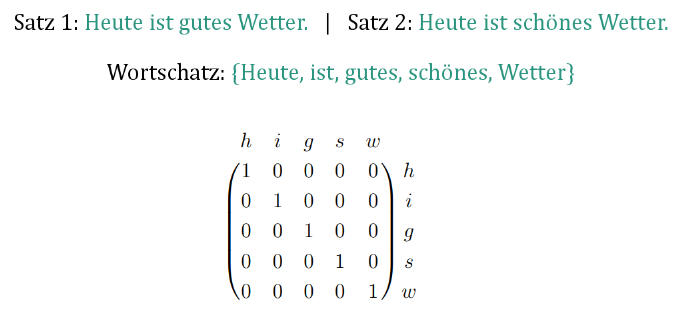
\includegraphics[width=0.65\linewidth]{./source/images/onehotencoding.png}}
  \caption{One-Hot-Encoding mit zwei beispielhaften Sätzen.}
  \label{pic:OneHotEncoding}
\end{figure}


\subsection{Bag-of-Words}
\noindent
\ac{BOW} realisieren die Feature Extraction, indem entsprechende Modelle das Aufkommen von in einem Wortschatz definierter Wörter über eine Vielzahl von Texten zählen. Dabei ist allerdings ein gewisser Informationsverlust zu erwarten, da beispielsweise die Reihenfolge der Wörter nicht berücksichtigt wird \cite[S.~262]{RAS19}. \autoref{table:BagOfWords} zeigt beispielhaft eine Matrix eines solchen \ac{BOW}-Modells.
\newpage

\noindent
In den Zeilen sind die betrachteten Texte indiziert, in den Spalten hingegen die Wörter des frei erfundenen Wortschatzes. Die Matrix hat demnach eine daran orientierte fixe Größe. In den Zellen ergeben sich somit die Häufigkeiten der Wörter, bezogen auf ihr Aufkommen in den einzelnen Texten \cite{BRO19}.

\begin{table}[htb]
\centering
\begin{tabular}{ | p{1.8cm} | p{1.8cm} | p{1.8cm} | p{1.8cm} | p{1.8cm} | p{1.8cm} | p{1.8cm} | p{1.8cm} | }
\hline
\textbf{ID} & \textbf{Heute} & \textbf{ist} & \textbf{schönes} & \textbf{Wetter} \\
\hline
Text 1 & 2 & 8 & 1 & 3 \\
\hline
Text 2 & 1 & 3 & 0 & 2 \\
\hline
Text 3 & 0 & 4 & 1 & 4 \\
\hline
\end{tabular}
\caption{Bag-of-Words mit einem beispielhaften Wortschatz \cite{HUI20}.}
\label{table:BagOfWords}
\end{table}

\noindent
Nachteilig ist dieser Ansatz hinsichtlich der \ac{ATS} insbesondere dadurch, dass die Reihenfolge der Wörter nicht berücksichtigt wird. Wie in \autoref{table:BagOfWords} ersichtlich wurde, lassen sich aus der Matrix keine Informationen über die Semantik oder Grammatik rekonstruieren. Aus technischer Sicht würde die Matrix bei steigender Wortschatzgröße nicht nur mitwachsen, sondern zudem viele Null-Einträge enthalten \cite{HUI20}. Vorteilig ist dieser Ansatz hingegen für eher schlichtere \ac{NLP}-Aufgaben. Hier sei die Klassifikation von Dokumenten als mögliches Einsatzgebiet genannt.


\subsection{Skip-Gram-Model}
\noindent
Ein weiterer frequenzbasierter Ansatz besteht in sogenannten Skip-Gram-Modellen. Diese unterliegen der Annahme, dass sich der Kontext eines gegebenen Wortes in Form von einer Textsequenz generieren lässt. Sei hierfür nun beispielhaft und gleichermaßen abstrakt die Sequenz {\{\textit{a, b, c, d, e}\}} gegeben. Zudem sei \textit{c} das Zielwort und die lokale Fenstergröße zwei. Ein Skip-Gram-Modell modelliert die bedingten Wahrscheinlichkeiten für die vor- und nachstehenden Kontextwörter \cite[S.~640]{ZHA20}. Hierfür gilt die folgende Formel: $$P(a, b, d, e \mid c)$$

\noindent
Gemäß der weitergehenden Annahme, die Kontextwörter ließen sich auf Grundlage eines gegebenen Zielwortes unabhängig voneinander generieren, kann die Formel wie folgt umgeschrieben werden: $$P(a \mid c) \cdot P(b \mid c) \cdot P(d \mid c) \cdot P(e \mid c)$$
\newpage

\noindent
Sei darüber hinaus abstrakter Wortschatz gegeben. Dabei erfordert jedes darin enthaltene Wort zwei mehrdimensionale Vektoren. Einen, um das Wort als Zielwort zu evaluieren, und einen, um das Wort in den unterschiedlichen Kontexten einzuordnen. Mithilfe dieser Vektoren können die bedingten Wahrscheinlichkeiten des entsprechenden Modells trainiert werden. Autark ist jedoch auch dieser Ansatz ungeeignet für die \ac{ATS} \cite[S.~641]{ZHA20}.


\subsection{Word2Vec}
\noindent
Der Ansatz des \ac{W2V} kombiniert \ac{BOW}-Modelle mit Skip-Gram-Modellen, um die Nachteile des \ac{OHE} weitergehend aufzuarbeiten. Dabei werden \ac{BOW}-Modelle jedoch in kontinuierlicher Form genutzt. Diese funktionieren in umgekehrter Weise zu den Skip-Gram-Modellen. Damit ist folglich eine beidseitige Herangehensweise möglich. Der Kontext kann also aus einem gegebenen Zielwort und das Zielwort wiederum aus einem gegebenen Kontext ermittelt werden \cite[S.~644]{ZHA20}.\\

\noindent
Die entsprechenden bedingten Wahrscheinlichkeiten können gemäß der nachstehenden Formeln modelliert werden. Dabei werden Skip-Gram-Modelle (erstgenannt) den \ac{BOW}-Modellen (zweitgenannt) anhand des oben genannten Beispiels gegenübergestellt. $$P(a, b, d, e \mid c) \qquad P(c \mid a, b, d, e)$$

\noindent
\ac{W2V}-Modelle können mithilfe neuronaler Netze trainiert werden. Dies befähigt sie, Zusammenhänge zwischen Wörtern zu erlernen. Hierbei werden Distanzen minimiert, die aus den zuvor beschriebenen Vektoren hervorgehen. Dieser Ansatz eignet sich in der Folge etwa dazu, Synonyme für gegebene Wörter zu bestimmen. \ac{ATS}-Modelle, welche den \ac{W2V}-Ansatz verfolgen, konnten sich in der Vergangenheit bereits in akzeptablem Maße beweisen \cite{KAR18}.\\

\noindent
\autoref{pic:OnlineSphere} zeigt die beispielhaften Projektionen von etwa 10.000 Wörtern, welche mit dem Embedding Projektor von TensorFlow und einer entsprechenden Hauptkomponentenanalyse generiert wurden. Dabei ist das Ergebnis der Suche nach dem Wort $play$ zu sehen. Es ist erkennbar, dass bedeutungsähnliche Wörter kürzere Distanzen aufweisen.
\newpage

\begin{figure}[h!]
  \centering
  \fbox{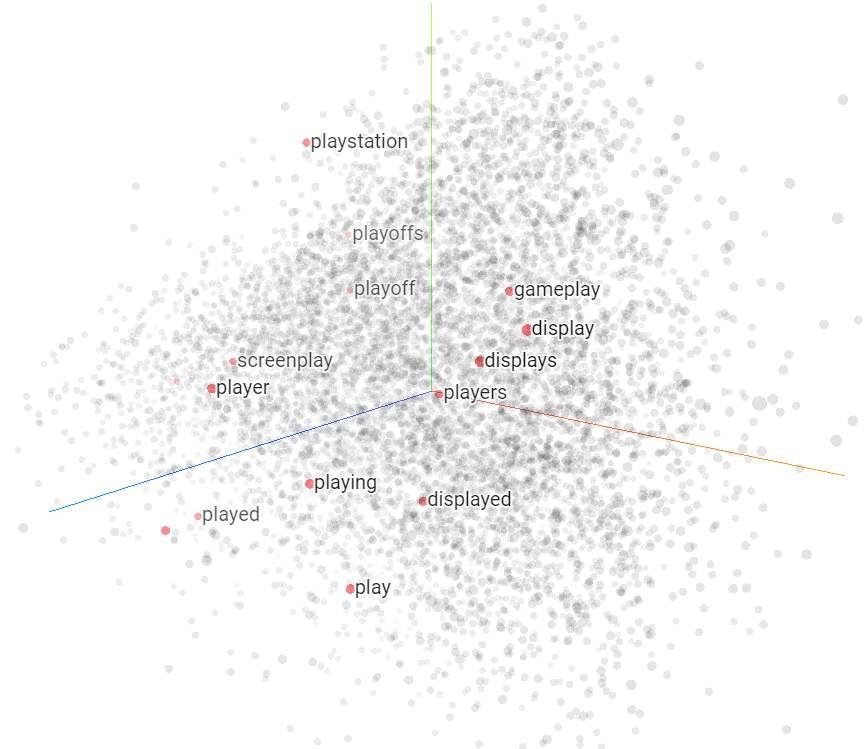
\includegraphics[width=0.75\linewidth]{./source/images/onlinesphere.png}}
  \caption{Word2Vec mit dem Embedding Projector von TensorFlow.}
  \label{pic:OnlineSphere}
\end{figure}


\subsection{Byte-Pair-Encoding}
\noindent
\ac{BPE} ist ein Algorithmus zur Datenkompression. Hierfür werden zusammenhängende Bytes mit einem Byte ersetzt, welches nicht in den sonstigen Daten auftritt \cite[S.~24]{NIT19}. Sei folgendes Beispiel gegeben: $$aaabcaacab = \boldsymbol{Z}\boldsymbol{Y}c\boldsymbol{Z}c\boldsymbol{Y}$$ $$\text{mit } \boldsymbol{Z} = aa \text{ und } \boldsymbol{Y} = ab$$

\noindent
\ac{BPE} eignet sich insbesondere dafür, seltene Wörter zu berücksichtigten. In diesen verbirgt sich mitunter eine nicht zu vernachlässigende Bedeutung. Aufgrund der kodierenden Funktion wird \ac{BPE} auch als Subword Embedding bezeichnet. Aufgrund der komprimierenden Funktion ist weiterhin von kleineren Modellgrößen auszugehen \cite[S.~24]{NIT19}. \ac{ATS}-Modelle, welche den \ac{W2V}-Ansatz verfolgen, konnten sich in der Vergangenheit ebenfalls in akzeptablem Maße beweisen.


\subsection{GloVe}
\noindent
\ac{GloVe} ist ein weiterer Algorithmus zur Einbettung von Texten in einen Vektorraum, welcher syntaktische und semantische Bedeutungen repräsentiert \cite[S.~1]{PEN14}.\\

\noindent
Hierfür wird sich einer Matrix bedient, welche das gemeinsame Aufkommen der im Korpus enthaltenen Wörter paarweise gegenüberstellt. Sie wird daher auch als Word-Word-Co-Occurrence-Matrix bezeichnet und besitzt eine maximale Komplexität von $O(|V|^2)$, wenn $V$ die Wortschatzgröße ist. \ac{GloVe} sieht dabei vor, die Matrix unter Nutzung lokaler Kontextfenster global zu faktorisieren \cite[S.~2]{PEN14}.\\

\noindent
Hierbei werden sehr große Matrizen durch mehrere niederrangige Matrizen approximiert. Dies ermöglicht es, die verborgenen statistischen Informationen des zugrundeliegenden Korpus anhand linearer Substrukturen zu explorieren und letztlich zu extrahieren. Dabei werden lokale Kontextfenster verwendet, wie sie bei verschiedenen oben genannten Ansätzen bereits beschrieben wurden, beispielsweise bei \ac{W2V} \cite[S.~24]{NIT19}.\\

\noindent
\ac{GloVe} ist praktisch als vortrainiertes Modell verfügbar. Dies basiert auf vier verschiedenen Korpora mit insgesamt etwa 55 Milliarden Token und einer durchschnittlichen Wortschatzgröße von etwa 1,5 Millionen Token. Im Training werden hierbei in der Matrix nur von Null verschiedene Werte berücksichtigt. Die mittlere quadratische Abweichung wird zudem als Fehlerfunktion ausgewählt. Das initiale Training ist zwar sehr rechenintensiv, dafür allerdings im Sinne des \ac{TL} a priori nur einmalig auszuführen. \ac{NLP}-Aufgaben, darunter auch die \ac{ATS}, profitierten stark vom Erfolg des \ac{GloVe}-Ansatzes. Trotzdem ist der Einsatz stets sorgfältig zu evaluieren, da innerhalb der modellinternen Vorverarbeitung die zugrundeliegenden Korpora beispielsweise auf Kleinschreibung forciert wurden. Dies müsste bei nachstehenden \ac{NLP}-Aufgaben ebenfalls berücksichtigt werden \cite[S.~6-9]{PEN14}.
\newpage


\section{Deep Language Representations}
\noindent
Die beschriebenen Word Embeddings verfolgen teils sehr abstrakte Ansätze, welche sich mitunter nur auf sehr wenige Teilbereiche des \ac{NLP} adaptieren lassen oder entscheidende Nachteile aufweisen. Zudem unterliegen sie meist statistischen und somit rechentechnischen Limitationen.\\

\noindent
\ac{ATS}-Modelle erfordern daher weitergehende \ac{DLR}, um den Anforderungen an das \ac{NLU} und die \ac{NLG} gerecht zu werden. Dabei werden die ursprünglichen Ansätze durch umfangreichere und komplexere neuronale Netze ersetzt. Diese werden fortan als Language Models bezeichnet. Nur wenige marktpräsente Akteure sind hierbei dazu fähig, geeignete Architekturen zu konzipieren und entsprechende Modelle von Grund auf neu zu trainieren. Dies wurde in der Vergangenheit bereits getan und veröffentlicht, sodass gemäß \ac{TL} nur noch ein weitergehendes Fine-Tuning nötig ist. Dabei profitierten nahezu alle nachstehenden \ac{NLP}-Aufgaben qualitativ von diesen Fortschritten. Architekturen, welche als \ac{DLR} zu verstehen sind und eine \ac{ATS} begünstigen, werden nachfolgend offengelegt \cite[S.~25]{NIT19}.


\subsection{ELMo}
\noindent
Zuerst sei \ac{ELMo} als Deep Contextualized Word Representation genannt. Es wurde vom Allen Institute for Artificial Intelligence entwickelt und 2018 veröffentlicht. \ac{ELMo} modelliert dabei einerseits komplexe Wortcharakteristiken wie Syntax und Semantik, andererseits aber auch den linguistischen Kontext eben dieser Wörter. Es ist als vortrainiertes Modell verfügbar und konnte nach der Veröffentlichung insbesondere \ac{NLU}-Aufgaben begünstigen \cite[S.~1]{PET18}.\\

\noindent
\ac{ELMo} arbeitet mit wortbezogenen kontextbasierten Vektoren, welche aus zwei bidirektionalen Language Models abgeleitet und trainiert werden. Diese bestehen wiederum aus zwei gekoppelten \ac{LSTM}-Schichten. Der umfangreiche Korpus an Textdaten wird dabei schichtweise vorwärts und rückwärts durch die Architektur propagiert. Somit sind kontextabhängige Informationen verfolgbar und die Bedeutungen der Wörter erlernbar. Aufgrund der zeichenbasierten Funktionsweise kann \ac{ELMo} sogar Wissen über Wortformen erlernen. Im Vergleich zu \ac{W2V} oder etwa \ac{GloVe} werden die Vektoren nicht tokenbasiert berechnet, sondern mithilfe einer Funktion, welche stets eine Sequenz berücksichtigt. Wörter können daher in verschiedenen Kontexten verschiedene Vektoren besitzen. \autoref{pic:ElmoStructure} visualisiert dies \cite[S.~2-3]{PET18}.

\begin{figure}[h!]
  \centering
  \fbox{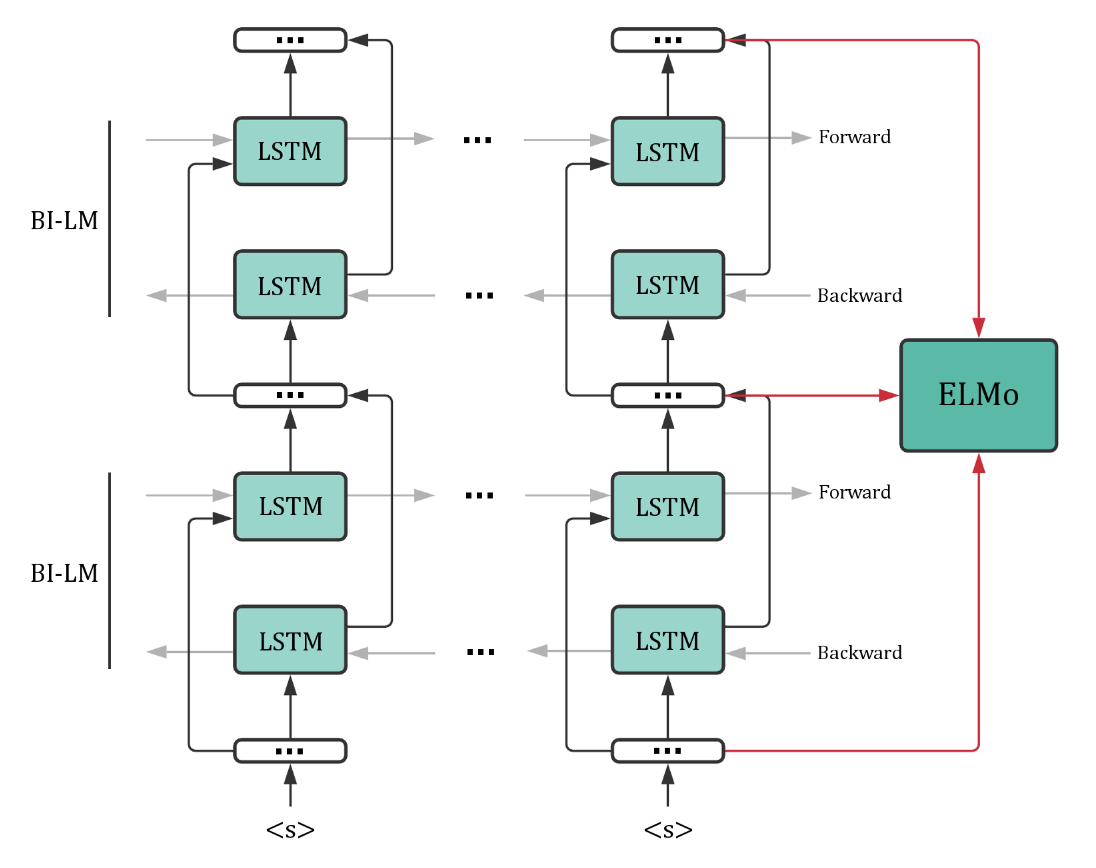
\includegraphics[width=0.7\linewidth]{./source/images/elmostructure.png}}
  \caption{Architektur und Funktionsweise von ELMo \cite{IRE18}.}
  \label{pic:ElmoStructure}
\end{figure}


\subsection{GPT}
\noindent
OpenAI arbeitet mit dem \ac{GPT} als Language Model in der nunmehr dritten Generation, veröffentlicht es allerdings nicht. Zu Forschungszwecken stellen sie dennoch eine schmalere Version des Modells bereit. OpenAI zeigt insbesondere mit dem \ac{GPT}, dass Language Models mithilfe der sogenannten Next Word Prediction besonders gut im Sinne des Unsupervised Learning trainiert werden können. Es basiert zudem auf der bereits bekannten Transformer-Architektur und begünstigt somit verschiedene nachgelagerte \ac{NLP}-Aufgaben, ohne entsprechende gelabelte Daten jemals gesehen zu haben. Dabei ist das \ac{GPT} meist besser als konkurrierende Modelle, welche auf den aufwendig zusammenzustellenden gelabelten Daten basieren, auch im sogenannten Zero-Shot-Transfer. Einer der größten Erfolge ist hierbei, dass das \ac{GPT} gemäß \ac{NLG} selbst einen Nachrichtenartikel verfassen konnte \cite[S.~1]{RAD19}.\\

\noindent
Die zugrundeliegenden Daten des \ac{GPT}-Modells bestehen aus 40GB an Texten, welche aus acht Millionen Internetseiten kollektiert wurden und zugleich bestimmten Qualitätsanforderungen gerecht werden. Hier nimmt OpenAI unter anderem an, dass Reddit-Beiträge mit einem ausreichend hohen positiven Karmastand eine erhöhte Qualität versprechen \cite[S.~3]{RAD19}.\\

\noindent
Im mathematischen Sinne wurde im Kontext der \ac{ATS} bislang meist die Wahrscheinlichkeit der Ausgabesequenz unter einer gegebenen Eingabesequenz modelliert. Language Models wie das \ac{GPT} streben hingegen ein allgemeineres Sprachverständnis an, um darüber hinaus eine Vielzahl an \ac{NLP}-Aufgaben unterstützen zu können. Daher modelliert das \ac{GPT} gemeinhin die Wahrscheinlichkeit $P(output \mid input, task)$ \cite[S.~2]{RAD19}. Aufgrund der eingeschränkten Verfügbarkeit seitens OpenAI entfallen an dieser Stelle weitere Ausführungen.


\subsection{BERT}
\noindent
Zudem sei \ac{BERT} als mögliches Modell zur \ac{DLR} genannt. Es wurde von Forschern der Google AI Language entwickelt und 2019 veröffentlicht. \ac{BERT} basiert auf ebenfalls der bereits bekannten Transformer-Architektur, wobei unstrukturierte Textdaten mithilfe links- und rechtsseitiger Kontextfenster bidirektional angelernt werden. Dabei entstammen die Daten verschiedenartigen \ac{NLP}-Aufgaben, sodass \ac{BERT} größtenteils aufgabenunabhängig einsetzbar ist. Im anschließenden Fine-Tuning werden die vortrainierten modellinternen Parameter zunächst initialisiert und wiederum mithilfe von gelabelten Daten angepasst. \ac{BERT} zeichnet sich weiterhin dadurch aus, dass er höchst anpassungsfähig ist und sich die vortrainierte Architektur nur minimal von der weitertrainierten Architektur unterscheidet \cite[S.~1-3]{DEV19}.\\

\noindent
Nun wird die Architektur von \ac{BERT} umfassender untersucht, indem die einleitenden Worte aufgegriffen und theoretisch ergründet werden. \ac{BERT} ist prinzipiell als Encoder zu verstehen, welcher durch einen mehrschichtigen bidirektionalen Transformer repräsentiert wird. Dabei werden die Schichten durch Transformer-Module repräsentiert. Diese verfügen über entsprechende Attention-Mechanismen, um kontextuelle Informationen zu erkennen. Weiterhin werden Sequenzen nicht nur einseitig betrachtet, sondern beidseitig, also bidirektional. Somit werden wortbezogene Kontexte gelernt, was insbesondere zu einem tieferen Verständnis der Sprache seitens \ac{BERT} führt. Dies ist ein großer Vorteil gegenüber bisheriger Architekturen, inklusive \ac{ELMo} und \ac{GPT}, welche Sequenzen zumeist nur einseitig betrachten konnten, also von links nach rechts oder andersherum. Aufgrund der qualitativen Vorteile von \ac{BERT} wird es umfänglicher als die ausgewählten Vorgänger und Konkurrenten analysiert \cite[S.~3]{DEV19}.
\newpage

\noindent
Um \ac{BERT} entsprechend vortrainieren zu können, werden \ac{MLM} genutzt. Bevor die Textdaten in die Architektur geführt werden, werden etwa 15\% der Wörter durch ein $[\text{MASK}]$-Token ersetzt. Daraufhin versucht das Modell, die maskierten Token auf Grundlage der umliegenden nicht-maskierten Token vorherzusagen (engl. Next Word Prediction). Da die zu erwartenden Wörter bekannt sind, kann über eine Klassifikationsschicht ein Lerneffekt erzielt werden, indem entsprechende Matrizen dimensional transformiert und wertmäßig aktualisiert werden. \autoref{pic:BertEncoder} zeigt die beschriebene Architektur \cite[S.~4-5]{DEV19}.\\

\begin{figure}[h!]
  \centering
  \fbox{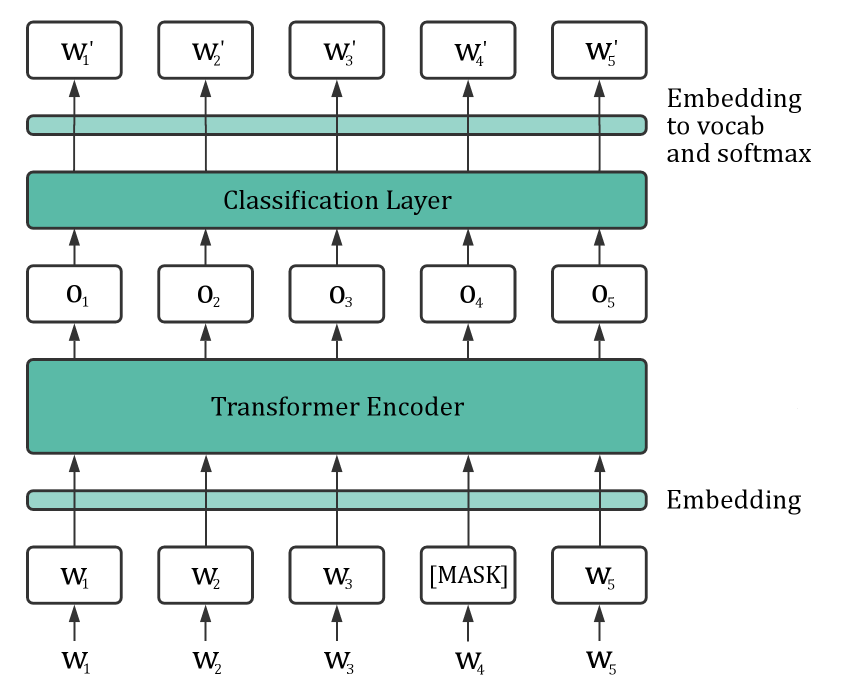
\includegraphics[width=0.65\linewidth]{./source/images/bertencoder.png}}
  \caption{Architektur von BERT mit MLM \cite[S.~3]{DEV19}.}
  \label{pic:BertEncoder}
\end{figure}

\noindent
Um zudem weitergehende Informationen auf Satzebene zu erhalten, werden dem Training paarweise Sätze zugeführt. Seien $A$ und $B$ zwei solcher Sätze, dann ist $B$ zu 50\% ein auf $A$ folgender Satz und zu 50\% ein zufälliger Satz des Korpus. Dies wird erneut im Sinne einer Klassifikation gelernt (engl. Next Sentence Prediction). Wie \ac{BERT} die eingehenden Sequenzen einbettet und repräsentiert, wird in \autoref{pic:InputRepresentation} deutlich. Dabei handelt es sich um die Summe der Token Embeddings, Segment Embeddings und Position Embeddings. Hierbei kann entschieden werden, ob Klein- und Großschreibung berücksichtigt werden soll \cite[S.~3-5]{DEV19}.
\newpage

\begin{figure}[h!]
  \centering
  \fbox{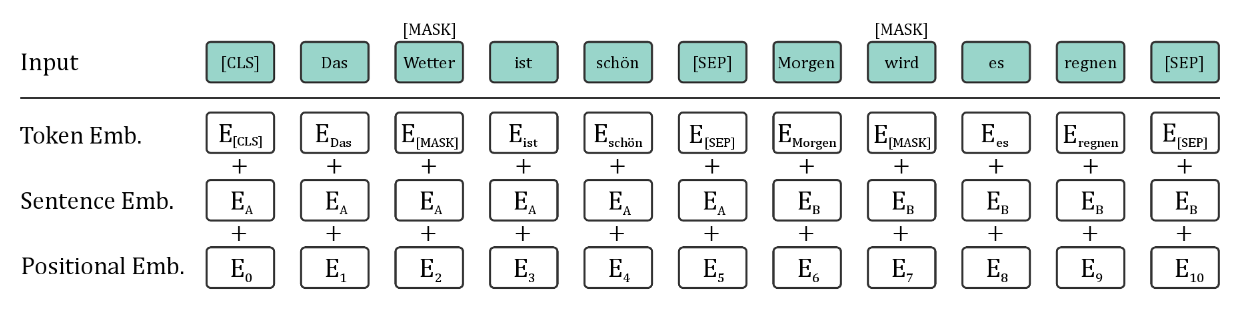
\includegraphics[width=0.95\linewidth]{./source/images/inputrepresentation.png}}
  \caption{Repräsentation von Textdaten mithilfe von BERT \cite[S.~3]{DEV19}.}
  \label{pic:InputRepresentation}
\end{figure}

\noindent
\ac{BERT} wurde initial in zwei verschiedenen Versionen veröffentlicht: BASE und LARGE. Die veröffentlichten Modelle wurden von den Forschern der Google AI Language auf zwei verschiedenen Korpora mit insgesamt über drei Millionen Wörtern trainiert. Sei $L$ die Anzahl der Schichten (oder: Transformer-Module), $H$ die Größe der verborgenen Schichten und $A$ die Anzahl der Self-Attention-Heads, dann sind die Versionen wie folgt definiert \cite[S.~3-5]{DEV19}. $$\text{BERT}_{\text{BASE}}: (L=12, H=768, A=12) \text{ mit } 110 \text{M Parametern}$$ $$\text{BERT}_{\text{LARGE}}: (L=24, H=1024, A=16) \text{ mit } 340 \text{M Parametern}$$


\subsection{XLM}
\noindent
\ac{XLM-R} ist ein weiteres Language Model, welches 2019 von Facebook AI veröffentlicht wurde und der Architektur von \ac{BERT} nahekommt. Es basiert demnach ebenfalls auf der bereits bekannten Transformer-Architektur. Es wird weiterhin über die Vorhersage absichtlich versteckter Textabschnitte unüberwacht trainiert. \ac{XLM-R} zeichnet sich insbesondere durch die multilinguale Funktionsweise aus. Hierfür wurde es auf mehr als zwei Terabyte an Textdaten vortrainiert, darunter Texte aus 100 verschiedenen Sprachen. Die Next Sentence Prediciton entfällt hingegen im Vergleich zu \ac{BERT}, während die \ac{LR} deutlich erhöht wird. Letztlich ist von \ac{XLM-R} durch die entsprechenden Anpassungen eine qualitative Verbesserung in verschiedenen \ac{NLP}-Aufgaben gegenüber der multilingualen Version von \ac{BERT} zu erwarten. Offensichtlich werden sprachübergreifende verborgene Strukturen erlernt, welche sich gegenseitig begünstigen. Darüber hinaus verwendet \ac{XLM-R} einen sprachübergreifenden Tokenizer. \ac{XLM-R} fordert Rechnern allerdings auch eine höhere Leistung ab \cite{CON20}.


\subsection{BART}
\noindent
\ac{BART} ist eine weitere Architektur der Facebook AI aus dem Jahre 2019, welche sich insbesondere für das Vortraining von Sequence-to-Sequence-Modellen eignet. Hierfür wird eingehender Text mithilfe einer Rauschfunktion verändert. Das Modell versucht daraufhin, den ursprünglichen Text zu rekonstruieren, um unüberwacht einen Lernfortschritt zu erzielen. \ac{BART} generalisiert bisherige Architekturen wie \ac{BERT} oder auch \ac{GPT}, weshalb es sich weiterhin um eine Transformer-Architektur handelt. Die besten Ergebnisse erzielte \ac{BART} in der jüngsten Vergangenheit bei \ac{NLG}-Aufgaben wie der \ac{ATS}, sowohl mono- als auch multilingual. Dabei schließt \ac{BART} qualitativ nicht nur zu \ac{XLM-R} auf, sondern übersteigt sie zu Teilen sogar \cite{LEW19}.


\section{Metriken}
\noindent
Weiterhin sind ausgewählte Metriken offenzulegen, mit denen die Qualität der \ac{ATS} gemessen werden kann: \ac{ROUGE} und \ac{BLEU}. In der Wissenschaft werden \ac{ATS}-Modelle meist mithilfe des \ac{ROUGE}-Scores evaluiert und verglichen. Dabei erfordern diese Metriken eine \ac{REFZ} zu jeder \ac{SYSZ}, welche maschinell generiert wurde. Dies ist unabhängig davon, ob das Training überwacht oder unüberwacht durchgeführt wird. Allgemein unterliegen diese Metriken der Herausforderung, dass es für einen gegebenen Text keine objektiv beste Zusammenfassung gibt. Folglich können verschiedene \ac{SYSZ} oder sogar \ac{REFZ} gleich gut sein. Dies ist statistisch sehr schwer zu bewerten, zumal selbst Menschen aufgrund ihrer subjektiven Bewertungsweise nicht einheitlich definieren können, welche Faktoren für eine gute Zusammenfassung stehen. Weiterhin werden in den Metriken menschliche Bewertungsfaktoren wie beispielsweise Lesbarkeit nicht berücksichtigt \cite{LEM20}.


\subsection{ROUGE}
\noindent
\ac{ROUGE} kann zunächst mithilfe folgender Kennzahlen weitergehend differenziert werden: Recall, Precision und Measure. Dabei quantifiziert der Recall-Score den Anteil der sowohl in \ac{REFZ} als auch in \ac{SYSZ} vorkommender Wörter gemäß folgender Formel:\\
$$\frac{\text{Anzahl übereinstimmender Wörter}}{\text{Anzahl der Wörter in der REFZ}}$$ \newline

\noindent
Sei hierfür verkürzt \glqq Der Sommer war sehr warm\grqq{} als \ac{REFZ} und \glqq Der Sommer war wieder sehr warm\grqq{} als \ac{SYSZ} gegeben. Dann gilt: $\text{Recall} = \frac{5}{5} = 1.0$. Trotzdem sollen \ac{SYSZ} nicht unendlich lang werden, um alle Wörter der \ac{REFZ} abzudecken, sondern weiterhin den eigentlichen Sinn einer Zusammenfassung erfüllen. Hier quantifiziert der Precision-Score den Anteil der tatsächlich relevanten Wörter gemäß folgender Formel:\\
$$\frac{\text{Anzahl übereinstimmender Wörter}}{\text{Anzahl der Wörter in der SYSZ}}$$ \newline

\noindent
Wie man sieht, ändert sich nur der Nenner. Im oben genannten Beispiel gilt somit: $\text{Precision} = \frac{5}{6} = 0.8\overline{3}$. Nimmt man ferner \glqq Der letzte Sommer war wieder sehr warm und trocken\grqq{} als neue \ac{SYSZ} an, dann reduziert sich der Precision-Score aufgrund der erhöhten Anzahl unrelevanter Wörter wie folgt: $\text{Precision} = \frac{5}{9} = 0.5\overline{5}$. Weiterhin kann der Measure-Score als gewöhnlicher F-Score verstanden und interpretiert werden. Er ergibt sich als harmonisches Mittel zwischen dem Recall und der Precision, womit er beide Scores berücksichtigt \cite[S.~1-3]{LIN04}.\\

\noindent
\ac{ROUGE} wird allgemein auch als \ac{ROUGE}-N geschrieben, wobei das N bestimmt, ob obige Kennzahlen auf Grundlagen von Uni-, Bi- oder Trigrammen berechnet werden sollen. Im genannten Beispiel wurden also die \ac{ROUGE}-1 Recall-, Precision- und Measure-Scores berechnet. Zudem existieren Ansätze, welche die \ac{LCS} verfolgen. Diese werden hier jedoch vernachlässigt.\\

\noindent
Trotz oder gerade wegen der wissenschaftlichen Verbreitung des \ac{ROUGE}-Scores kommt immer mehr Kritik auf. Demnach kann \ac{ROUGE} beispielsweise nicht zwischen verschiedenen aber bedeutungsähnlichen Wörtern unterscheiden. Dies führt tendenziell zu einer schlechteren Bewertung, obgleich ein gegebener Text etwa in einer entsprechenden \ac{SYSZ} präzise zusammengefasst wurde. Außerdem wird den Texten zur Berechnung des \ac{ROUGE}-Scores Kleinschreibung abverlangt, unabhängig von den vorgeschalteten Modellen. Die Bewertung geschieht also eher auf syntaktischer als auf semantischer Basis. Aufgrund der bereits genannten weitreichenden Nutzung des \ac{ROUGE}-Scores und der damit gegebenen Vergleichbarkeit kommt er trotzdem in dieser Arbeit zum Einsatz \cite[S.~5]{LIN04}.

	
\subsection{BLEU}
\noindent
\ac{BLEU} kommt der Funktionsweise von \ac{ROUGE} weitestgehend gleich. Demnach repräsentiert der Score ebenfalls die Ähnlichkeit längendefinierter N-Gramme. Dabei wird weiterhin für jede \ac{SYSZ} eine entsprechende \ac{REFZ} gefordert. Beide Metriken funktionieren indes sprachunabhängig. Im Unterschied zu \ac{ROUGE} führt \ac{BLEU} einen multiplikativen Bestrafungsterm ein, um zu kurze \ac{SYSZ} zu entwerten. Dies ist nicht notwendig, wenn die \ac{SYSZ} länger ist als die \ac{REFZ}. Der Precision-Score berücksichtigt dies bereits \cite[S.~5]{PAP02}.\\

\noindent
Obgleich der \ac{BLEU}-Score primär die Bewertung von Übersetzungen unterstützt, eignet er sich gewissermaßen auch für \ac{ATS}-Aufgaben. Zuletzt konnte wissenschaftlich bewiesen werden, dass der \ac{BLEU}-Score recht gut mit menschlichen Bewertungen korreliert. Aufgrund ähnelnder Nachteile zu denen des \ac{ROUGE}-Score und fehlender wissenschaftlicher Vergleichbarkeit wird der \ac{BLEU}-Score in dieser Arbeit nicht verwendet \cite[S.~6-7]{PAP02}.
